\documentclass[10pt]{article}
\usepackage[utf8]{inputenc}
\usepackage[T1]{fontenc}
\usepackage[french]{babel}
\usepackage{graphicx}
\usepackage{hyperref}
\title{Titre}
\author{Nathan Marotte}
\begin{document}
\maketitle
\section{Introduction}
Le vaccin est au coeur des débats ces dernières années avec la montée du mouvement \textit{anti-vaxx}, principalement aux Etats-Unis, qui se base sur diverses croyances, notamment l'autisme soi-disant causé par certains vaccins, la toxicité de certains vaccins, ou encore l'innéficacité des vaccins, uniquement distribués pour remplir les poches des lobbies pharmaciautiques. C'est surtout de ce dernier point que l'on va discuter dans cet article. Nous allons voir comment fonctionne les vaccins, ainsi que leur différentes efficacité en fonction de la maladie et des caractéristiques de la population.

\section{Danger des vaccins}


\subsection{Comme cause de l'autisme}
L'autisme est un trouble du développement caractérisé par des problèmes de communication et d'interactions sociales. Les causes de cette maladie, bien que toujours sujettes à la recherche, s'oriente principalement vers des facteurs génétiques \cite{genetics} et une infection virale de la mère pendant la grossesse \cite{autism_viral}\cite{genetic_evaluation}. La communauté scientifique à refuté les vaccins comme cause d'autisme à plusieurs reprises [4][5][6]

\subsection{composé de matériaux toxiques}
Le thiomersal est un composé organique utilisé comme conservateur dans certains vaccins et est la principale cause de panique sur les vaccins. Sa composition chimique contenant du Mercure pourrait donner une impression de toxicité mais il n'y a pas de preuve scientifique supportant cette idée.[7] Ce composé est utilisé pour empêcher le développement de bactéries dans dans les vaccins et a une durée de demi-vie de 6.9 jours dans le sang, ce qui est bien moindre que la durée de demi-vie moyenne des composés méthylmercure [8]

\section{Efficacité des vaccins}
\subsection{Principe}
Les vaccins servent d'entrainement pour notre système immunitaire. Ils consistent en l'injection d'une faible quantité d'un agent infectieux, virus ou bactérie, atténué ou mort afin d'enclencher une réponse immunitaire de l'individu et permet de gagner facilement le combat contre cette infection. Ce processus génere des cellules mémoire dans notre système immunitaire qui permettront à notre organisme de réagir plus vite et plus efficacement lors d'une prochaine infection.
\subsection{Efficacité individuelle}
Du fait de la réaction immunitaire enclenchée par la prise du vaccin, notre corps tire de cet évenement un bénéfice non négligable. Lors d'une infection bactérienne, les individus précédemment vaccinés sont hôte d'un nombre bien plus faible de de colonies que les individus non vaccinés [9]. Dans le cas des infections virales, avec le rhume par exemple, les individus vaccinés présentent en moins grande fréquence les symptômes de la maladie [10]
\subsection{Efficacité sur la population}
Lorsqu'un individu précédemment vacciné est infecté par un virus ou une bactérie reconnue par son système immunitaire, du fait que l'infection soit combattue plus rapidement et efficacement, il en résulte en une diminution de la transmission du virus à un autre individu [11]. C'est de cette réduction de transmission que nous allons parler dans cet article.

\section{La façon dont une population vaccinée est protégée au delà de l'individu}
\subsection{Introduction}
En considérant une population de 2500 individus vaccinée à un certain pourcentage comme terrain de chasse d'une maladie très infectieuse ($R_0=8$), avec un taux de mortalité nul et un temps de guérison infini, nous pouvons simuler assez facilement la propagation de cette maladie avec un modèle SI et comparer le taux de vaccination de la population avec le nombre d'individu ayant été épargné de la maladie. Ces taux ont été choisi pour simplifier le modèle pour faire apparaître ce qui nous intéresse ici, la façon dont la maladie se propage dans la population et si elle peut être arrêtée par des personnes vaccinées.
\subsection{Symboles et constantes}
Nous utiliserons $V$ pour la probabilité que chaque individu a d'être vacciné. Cette probabilité est ensuite multiplié par le nombre d'individu afin d'avoir un nombre exact de personnes à vacciner. $V \in [0,1]$
La population sujette à l'infection est approximée par un carré de 50 individus de coté sans mouvement, mort d'individu, ou guérison de la maladie.
La maladie que nous allons appellée Sissi suit un modèle SI avec comme nombre d'infecté au temps 0 $I_0 = 1$, le nombre de personne qu'un infecté peut infecter est $R_0 = 8$ (dans le cas ou les voisins ne sont pas déjà infecté, sinon il peut-être inférieur), la probabilité de transmission $\alpha = 1$, la probabilité de guérison $\beta = 0.00$, et la probabilité de mort $\delta = 0.00$.

\subsection{Résultats}
\label{sec:results}
En faisant la moyenne sur 5000 itérations par $V$ nous obtenons assez de données pour créer un graphe comparant le pourcentage de vaccinés au pourcentage de personnes susceptibles au départ touchées par la maladie et mets en évidence l'immunité collective qui permet à une population d'être protégée à 95\% lorsque vaccinée aux alentours de 67\%, dans notre modèle.
Si $R_0$ augmente, pour atteindre notre \textit{threshold} de 95\%, la population devra être vaccinée à un plus haut pourcentage vu qu'il faudra plus que plus de 8 voisins soient vaccinés pour être protégé (voir discussions)

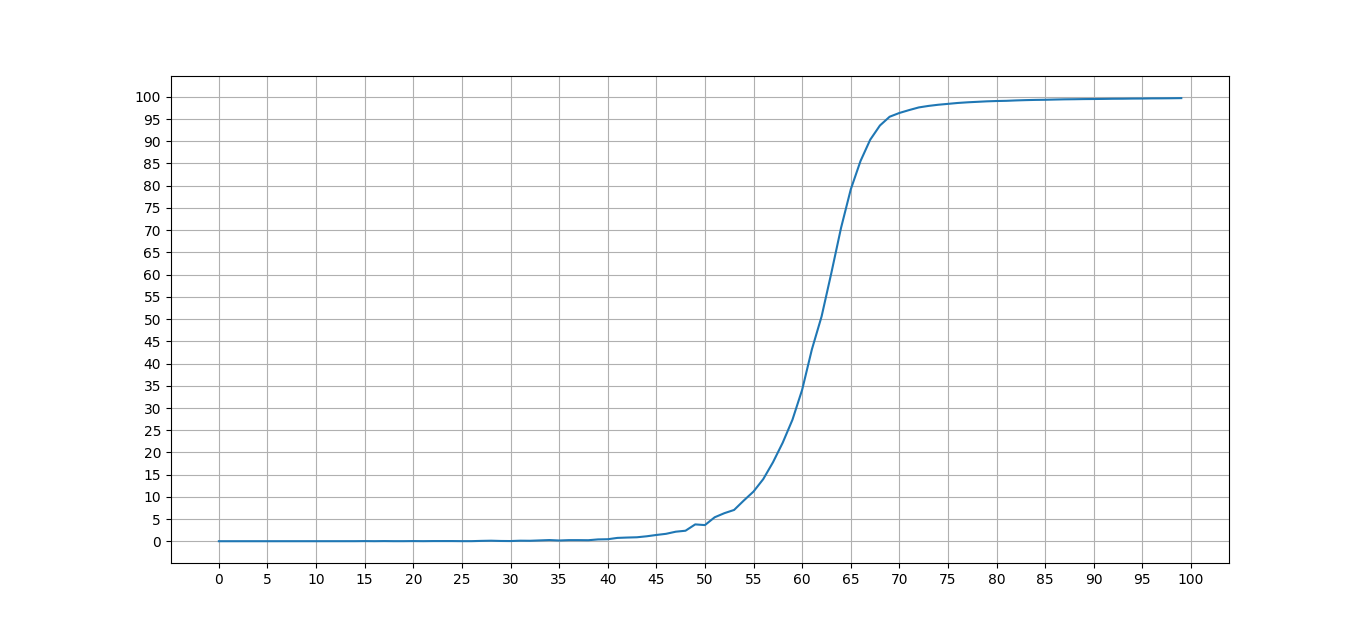
\includegraphics[scale=0.3]{5000iter.png}


\subsection{Matériel et méthode}
\subsubsection{Modèle}
Notre simulation se base sur un cas particulier du modèle SIR où la probabilité de passer d'infecté (I) à soigné (R) est de 0. Certains individu commencent sur l'état R. On dit qu'ils sont vaccinés, et sont donc, dans notre modèle, insensible à la contagion. Les autres individus commencent sur l'état susceptible (S) sauf $I_0$ individu qui commencent dans l'état I.
\subsubsection{Matrice}
Les individus de notre simulation sont approximés par une matrice carrée de 50 lignes composée chacune de 50 entrées pour 2500 individus au total. Chaque entrée de la matrice correspond à l'état d'un individu. 0 pour susceptible (S), 1 pour infecté (I) et 2 pour vaccinné (R)
\subsubsection{Propagation}
Notre simulation tourne étape par étape. A chaque étape de la propagation, nous allons d'abord décider si il y a plus d'infecté que de susceptible, si c'est le cas, alors nous allons regarder les voisins de chaque individu susceptible. Si ce voisin est infecté, on tire un chiffre au hasard suivant une loi de probabilité uniforme et si ce chiffre est inférieur à $\alpha$, alors nous infectons l'individu susceptible. Si par contre il y a plus de susceptibles que d'infecté, alors nous allons parcourir les infecté, et pour chaque voisin susceptible, nous tirons un chiffre au hasard suivant la même loi de probabilité et on infecte ce voisin si le chiffre est inférieur à $\alpha$. Cette distinction de deux états du modèle (plus d'infecté, ou plus de susceptible) permet de réduire le nombre de calcul dans les cas déséquilibrés.
La simulation s'arrête lorsqu'il n'y a plus de nouveaux infectés. Cette condition d'arrêt n'est bonne que dans le cas où $\alpha = 1$, sinon on peut s'arrêter soit après un certain nombre de jour, soit lorsque le nombre de personnes susceptibles dans le voisinage de tous les infectés est de 0, soit lorsque la maladie est éradiquée dans le cas où $\beta > 0$ ou $\delta > 0 $


\subsubsection{Probabilité qu'un individu aie k voisins vaccinés}
Cette probabilité est calculée facilement en utilisant une loi de probabilité binomiale $$P(X = k) = B(n;p) = {n \choose k}\times p^k \times q^{n-k} = \frac{n!}{k!(n-k)!}\times p^k \times q^{n-k}$$ où $X$ est notre variable aléatoire, $k$ est le nombre de voisins vacciné, $n$ est le nombre de voisins et $p$ la probabilité pour un voisin d'avoir été vacciné. En appliquant cette formule pour $k$ allant de 1 à 8 inclus, le cas 0 étant trivial, et pour p allant de 0 à 100 inclus, nous obtenons ce graphique nous donnant la probabilité qu'un individu soit enouré par 1 à 8 vacciné en foncton du pourcentage de vaccinés. Cette formule et le graphe correspondant nous permet de trouver des informations comme par exemple : dans une population vaccinée à 50\%, la probabilité qu'un individu possède 8 voisins vaccinés est d'environ 0.39\%.

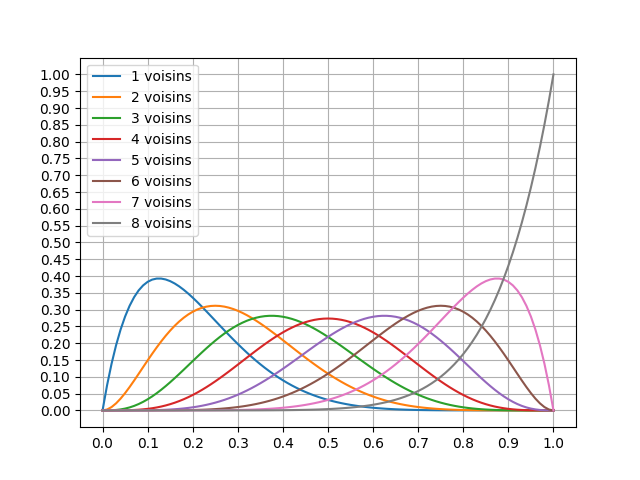
\includegraphics[scale=0.6]{probNeighbour.png}

\subsubsection{Obtention des résultats}
Afin d'obtenir le graphique \ref{sec:results}, nous avons exécuté notre algorithme 500.000 au total. Pour chaque pourcentage de vaccination de 0 à 99 inclus, nous avons exécuter 5000 simulations complètes. Nous avons ensuite fait la moyenne du nombre d'individu susceptibles à la fin de chacune de ces 5000 itérations.
Après avoir récolté ces données, nous avons d'abord divisé ce nombre par le nombre d'individu susceptible au départ, ce qui correspond à $2500-V*25-1$. 2500 individus au départ, moins 25 par pourcentage de vacciné moins $I_0$



\begin{thebibliography}{9}

\bibitem{genetics}
C M Freitag.
\href{https://doi.org/10.1038/sj.mp.4001896}{The genetics of autistic disorders and its clinical relevance: a review of the literature} (https://doi.org/10.1038/sj.mp.4001896)

\bibitem{autism_viral}
Jane E. Libbey, Thayne L. Sweeten, William M. McMahon \& Robert S. Fujinami
\href{https://doi.org/10.1080/13550280590900553}{Autistic disorder and viral infections} (https://doi.org/10.1080/13550280590900553)

\bibitem{genetic_evaluation}
Nancy J.Mendelsohn, G. BradleySchaefer
\href{https://doi.org/10.1016/j.spen.2008.01.005}{Genetic Evaluation of Autism} (https://doi.org/10.1016/j.spen.2008.01.005)

\bibitem{develop_disorder_immunizations}
Eric Fombonne, Rita Zakarian, Andrew Bennett, Linyan Meng and Diane McLean-Heywood
\href{https://doi.org/10.1542/peds.2005-2993}{Pervasive Developmental Disorders in Montreal, Quebec, Canada: Prevalence and Links With Immunizations} (https://doi.org/10.1542/peds.2005-2993)

\bibitem{vaccine_wars}
Liza Gross
\href{https://doi.org/10.1371/journal.pbio.1000114}{A Broken Trust: Lessons from the Vaccine–Autism Wars} (https://doi.org/10.1371/journal.pbio.1000114)

\bibitem{evidence_based}
Luke E.Taylor, Amy L.Swerdfeger, Guy D.Eslick
\href{https://doi.org/10.1016/j.vaccine.2014.04.085}{Vaccines are not associated with autism: An evidence-based meta-analysis of case-control and cohort studies} (https://doi.org/10.1016/j.vaccine.2014.04.085)

\bibitem{vaccines_do_not_cause_autism}
Center for Diseases Control and Prevention (CDC) : The leading national public health institute of the United States of America
\href{https://www.cdc.gov/vaccinesafety/concerns/autism.html}{Vaccines do not cause autism}

\bibitem{Thimerosal}
Julia R. Barret
\href{https://www.ncbi.nlm.nih.gov/pmc/articles/PMC1280369/}{Thimerosal and Animal Brains: New Data for Assessing Human Ethylmercury Risk}

\bibitem{Experimental infection of bacteria}
R.A.Juste, J.F.García Marín,, B.Peris, C.Sáez de Ocáriz, J.J.Badiola
\href{https://doi.org/10.1016/S0021-9975(08)80189-2}{Experimental infection of vaccinated and non-vaccinated lambs with Mycobacterium paratuberculosis}

\bibitem{Immune response Sweden 2009}
Isabelle Magalhaes, Mikael Eriksson, Charlotte Linde, Rashid Muhammad, Lalit Rane, Aditya Ambati, Rebecca Axelsson-Robertson, Bahareh Khalaj, Nancy Alvarez-Corrales, Giulia Lapini, Emanuele Montomoli, Annika Linde, Nancy L Pedersen, Markus Maeurer
\href{https://doi.org/10.1186/1471-2334-14-319}{Difference in immune response in vaccinated and unvaccinated Swedish individuals after the 2009 influenza pandemic}

\bibitem{vaccine-induced reduction in virus transmission}
Mart C.M.De Jong, Tjeerd G.Kimman
\href{https://doi.org/10.1016/0264-410X(94)90229-1}{Experimental quantification of vaccine-induced reduction in virus transmission}
\end{thebibliography}






\end{document}
